\section{Architectures}
In questa prima sezione verranno esaminate le varie architetture che sono state progettate e sintetizzate per il moltiplicatore floating point

\subsection{Classic Architecture}
Il punto di partenza della progettazione è stato il floating point pipelined multiplier a 32 bit, del quale è stato fornito il codice vhdl.
Lo schema di massima è mostrato in \autoref{fig:mult_struct}, è suddiviso in 4 stage principali:
\begin{itemize}
\item Stage 1: Viene effettuato l'unpacking dei due numeri floating point in ingresso.
\item Stage 2: Viene effettuata la moltiplicazione dei significands, trattati come numeri interi.
\item Stage 3: Viene effettuato il rounding dei significands.
\item Stage 4: Viene effettuato il calcolo dell'esponente e infine viene trasformato nuovamente il numero in floating point tramite il blocco di packing.
\end{itemize}

\begin{figure}[h]
	\center
	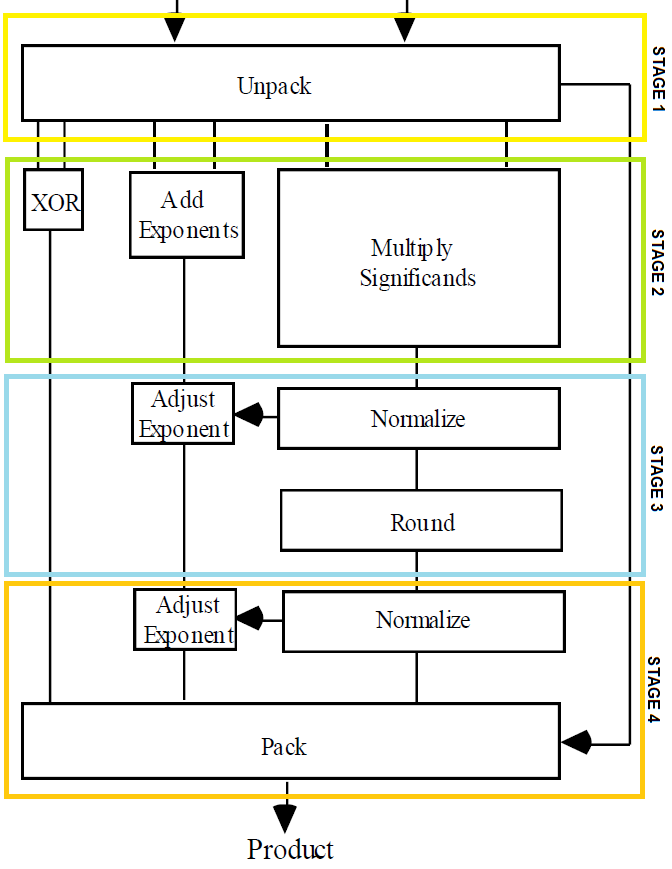
\includegraphics[width=0.6\textwidth]{mult_structure.png}
	\caption{Structure of the floating point multiplier}
	\label{fig:mult_struct}
\end{figure}

\noindent Studiando il codice VHDL si nota inolte che tra uno stadio e l'altro sono sempre presenti dei registri che campionano il segnale sul fronte di salita del clock. Per questo si può affermare che gli stage funzionali corrispondono agli stage di pipeline.
\todo{E'GIUSTO?}
Un'altra osservazione che è possibile fare su questa architettura standard è che nel secondo stage, il tipo di moltiplicatore utilizzato per moltiplicare i significands non è specificato infatti è presente un process nel quale viene fatta l'operazione con il simbolo "*" che lascia completa libertà al sintetizzatore nella scelta dell'implementazione hardware.

\subsubsection{Testbench}

Prima di partire con le varie modifiche dell'hardware è stato simulato tramite Modelsim il corretto funzionamento del circuito fornito. E' stato creato un testbench in verilog con i blocchi relativi alla generazione degli input, al DUT e al salvataggio degli output.
Come file di ingresso è stato utilizzato quello fornito sia per l'ingresso $A$ sia per $B$ di conseguenza il moltiplicatore effettuava il quadrato del numero in questione. I numeri erano rappresentati su 8 bit esadecimali quindi prima di fornirli al DUT è stata effettuata la conversione in binario.
Infine, confrontando i risultati ottenuti con quelli forniti come esempio, è stato possibile confermare il funzionamento del circuito. Inoltre studiando il timing generato da Modelsim si nota come effettivamente la latenza del circuito sia quella ipotizzata.
\\
\todo{GIUSTO?}
Successivamente è stato modificato il codice VHDL in modo da aggiungere ai segnali di ingresso dei registri; questa correzione serve a svincolare il timing degli ingressi, con eventuali glitch, dal timing interno del circuito.
A fronte di questa modifica è stato effettuato un secondo testbench, funzionalmente uguale al precedente, che ha mostrato anche in questo caso che il circuito sotto esame funzionasse correttamente.

%%%%%%%%%%%%%%STAGE 2 MANIPULATION%%%%%%%%%%%%%%%

\subsection{Stage 2 CSA PPARCH}
In this section a few optimizations were done. In fact, compared to the classic architecture there are several differences that change the circuit behavior. The CSA architecture is implemented by using the \textit{Carry Save Adders} and in the PPARCH architecture there is a \textit{Parallel Prefix} version of the stage 2. These variations can be simply carried out by using different commands during the compilation process. The stage 2 was forced to be syntetized as CSA and in order to do that the following commands were used in the synthesis process:
\begin{itemize}
\item ungroup -all flatten
\item set\_implementation DW02\_mult/csa [find cell *mult] 
\end{itemize}
For the PPARCH the same commands were used, but with one difference in the mult options:
\begin{itemize}
\item ungroup -all flatten
\item set\_implementation DW02\_mult/pparch [find cell *mult] 
\end{itemize}
The goals of the synthesis process was the area and the minimum period estimation and the results obtained from the commands \textit{report\_area} e \textit{report\_timing} are showed in \autoref{tab:syn_results}: the \textit{CSA} architecture is roughly three times slower and the area is much greater than the \textit{PPARCH} one and the \textit{PPARCH} is a better architecture respect to the \textit{CSA} one.
To check the correct behavior, a testbench was performed on both architectures, and the otuput is shown in the following table:

\begin{table}[H]
\begin{center}
\begin{tabular}{|c|c|c|c|}				\hline
CSA		 	  & PPARCH 					\\ \hline
00000000   	  & 00000000               	\\ \hline
3DC3910D      & 3DC3910D                \\ \hline
0BC80005      & 0BC80005                \\ \hline
3F278DDF      & 3F278DDF                \\ \hline
0B100005      & 0B100005                  \\ \hline
3F800000      & 3F800000              \\ \hline
0C440004      & 0C440004                 \\ \hline
3F278DDF      & 3F278DDF                 \\ \hline
0DA20000      & 0DA20000                   \\ \hline
3DC3910D      & 3DC3910D                 \\ \hline
3DC3910D      & 3DC3910D                   \\ \hline
3DC3910D      & 3DC3910D                   \\ \hline
\end{tabular}
\end{center}
\end{table}

As the table illustrates, the behavior of both architecture is the same; in addiction, once the input stream reaches the end of file, the output remains the same as long as the simulation runs, in fact the output remains equal to the string \textit{3DC3910D}. In conclusion both architectures work, but in a different way due to the internal structure.

%%%%%%%%%FINE-GRAIN PIPELINING%%%%%%%%%%%%%

\subsection{Fine grain pipelining}
The next aim is to modify the VHDL file by inserting a \textit{pipeline stage} in stage 2 output, as shown in the following image:
\begin{figure}[H]
	\center
	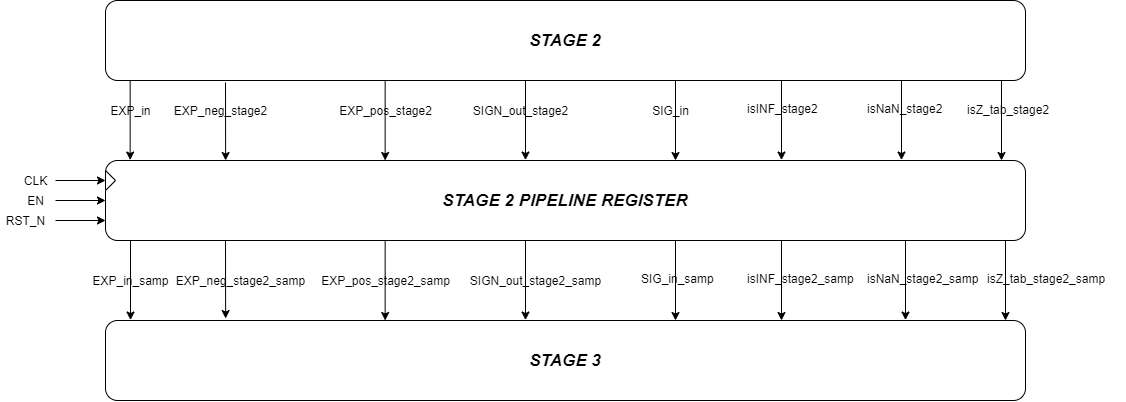
\includegraphics[width=0.9\textwidth]{Fine grain pipelining.png}
	\caption{Fine grain pipelining block diagram}
	\label{fig:mult_struct}
\end{figure}
The output register has been implemented in the VHDL file by using several registers and \textit{flip-flops} in order to ensure the correct behavior and timing.  After the VHDL manipulation, two different synthesis processes were made by using different commands per time: in the first run, the compile command was launched after \textit{optimize\_registers} command and in the second run  \textit{compile\_ultra} was used rather than \textit{optimize\_registers} and \textit{compile}. The Synthetizer elaborates the structures in a different way, by using some algorithms instead of other ones, according to the choosen command. The results in terms of timing and area are showed in \autoref{tab:syn_results}: the \textit{compile\_ultra} give a lower area but the circuit is clearly slower respect to the one obtained by using \textit{optimize\_registers}.


\subsection{Modified Booth Encoding (MBE)}
The Modified Booth Encoding Multiplier is an extension of the Radix-2 approach, where a Radix-4 approach is used in order to produce half partial products. In generale considerando \textbf{a} e \textbf{b} come due numeri unsigned nella forma seguente:
$$
\textbf{a} = \sum_{i=0}^{n-1}a_i2^i\ \ \ \ \ \ \  \textbf{b} = \sum_{i=0}^{n-1}b_i2^i
$$
The product \textbf{c} is obtained:
$$
\textbf{c} = \sum_{i=0}^{n-1}\sum_{i=0}^{n-1}a_ib_i2^{i+j}
$$
Radix-2 approach produces \textbf{n} partial products in the form:
$$
p_j = 
\begin{cases}
0 \ \textrm{  if   } \overline{b}_j\\
a \ \textrm{  if   } {b}_j
\end{cases}
$$
On the other hand MBE produces only \textbf{n/2} partial products because more bits are analyzed simultaneously. The multiplier is divided in 3-bit slices (with $b_{-1} = 0$), where two consecutive slices feature a 1-bit overlap. Then, each triplet of bits is exploited to encode the multiplicand according to the \autoref{tab:MBE}.

\begin{table}[htb]
	\centering
	\begin{tabular}{cc}
		$b_{2j+1}b_{2j}b_{2j-1}$ & $p_j$ \\ 
		\hline 
		000 & 0 \\ 
		001 & a \\ 
		010 & a \\ 
		011 & 2a \\ 
		100 & -2a \\ 
		101 & -a \\ 
		110 & -a \\ 
		111 & 0 \\ 
	\end{tabular}  
	\label{tab:MBE}
	\caption{Modified Booth Encoding}
\end{table}
The expression to evaluate $p_j$ is $p_j = (b_{2j+1} \oplus q_j) + b_{2j+1}$ where
$$ q_j=
\begin{cases}
0 \ \textbf{  if   } (\overline{b_{2j} \oplus b_{2j-1}})(\overline{b_{2j+1} \oplus b_{2j}})\\
a \ \textbf{  if   } b_{2j} \oplus b_{2j-1}\\
2a \ \textbf{  if   } (\overline{b_{2j} \oplus b_{2j-1}})(b_{2j+1} \oplus b_{2j})
\end{cases}
$$
Sono stati utilizzati 16 blocchi combinatori per valutare tutti i prodotti parziali che devono essere sommati. Una visione d'insieme della struttura con na visualizzazione a punti si può osservare in \autoref{fig:Dadda_1}

\begin{figure}[htb]
	\center
	
\includegraphics[width=1\textwidth]{Dadda_Tree_1.png}
	\caption{Partial products representation}
	\label{fig:Dadda_1}
\end{figure}
Per coprire i bit si è usato un Dadda Tree in modo da usare un numero ottimale di stadi e quindi una velocità elevata nell'eseguire le operazioni. L'approccio consiste nel ridurre l'altezza ad ogni stadio fino a raggiungere un numero di bit prefissato utilizzando half-adder e full-adder. Le altezze seguono la sequenza:
$$
d_1 = 2 \ \ \ \ \ \ \ \ d_{j+1} = \lfloor(1.5d_j)\rfloor
$$
L'altezza iniziale della struttura è pari a 16, quindi la sequenza sarà:
$$
d_1 = 2,\ d_2 = 3,\ d_3 = 4,\ 
d_4 = 6,\ d_5 = 9,\ d_6 = 13,\ d_7 = 16
$$
Avendo lo step successivo un'altezza di 13, tutte le colonne che presentano un numero maggiore di bit devono essere ridotte. Partendo da destra, sulla prima colonna che ha 14 bit è stato inserito un half-adder che a partire da due bit genera un nuovo bit sulla stessa colonna e uno di carry sulla colonna successiva. La colonna adiacente che ha ancora 14 bit, considerando il riporto proveniente dal half-adder precedente, necessita un full-adder che a sua volta genera un bit di somma sulla stessa colonna e un bit di carry sulla colonna successiva partendo da tre bit. Questo ragionamento è stato ripetuto su tutta la struttura e il risultato finale è osservabile in \autoref{fig:Dadda_1} in cui sono stati impiegati 6 half-adder (in arancio) e 33 full-adder (in verde).\\
Lo stesso meccanismo viene applicato ad ogni stadio per ridurre il numero di bit rispettando la sequenza. In \autoref{fig:Dadda_2} è possibile osservare la copertura di ogni stadio fino ad avere un'altezza di due bit, dove grazie ad un sommatore si può computare il risultato finale. 

\begin{figure}[htb]
	\center
	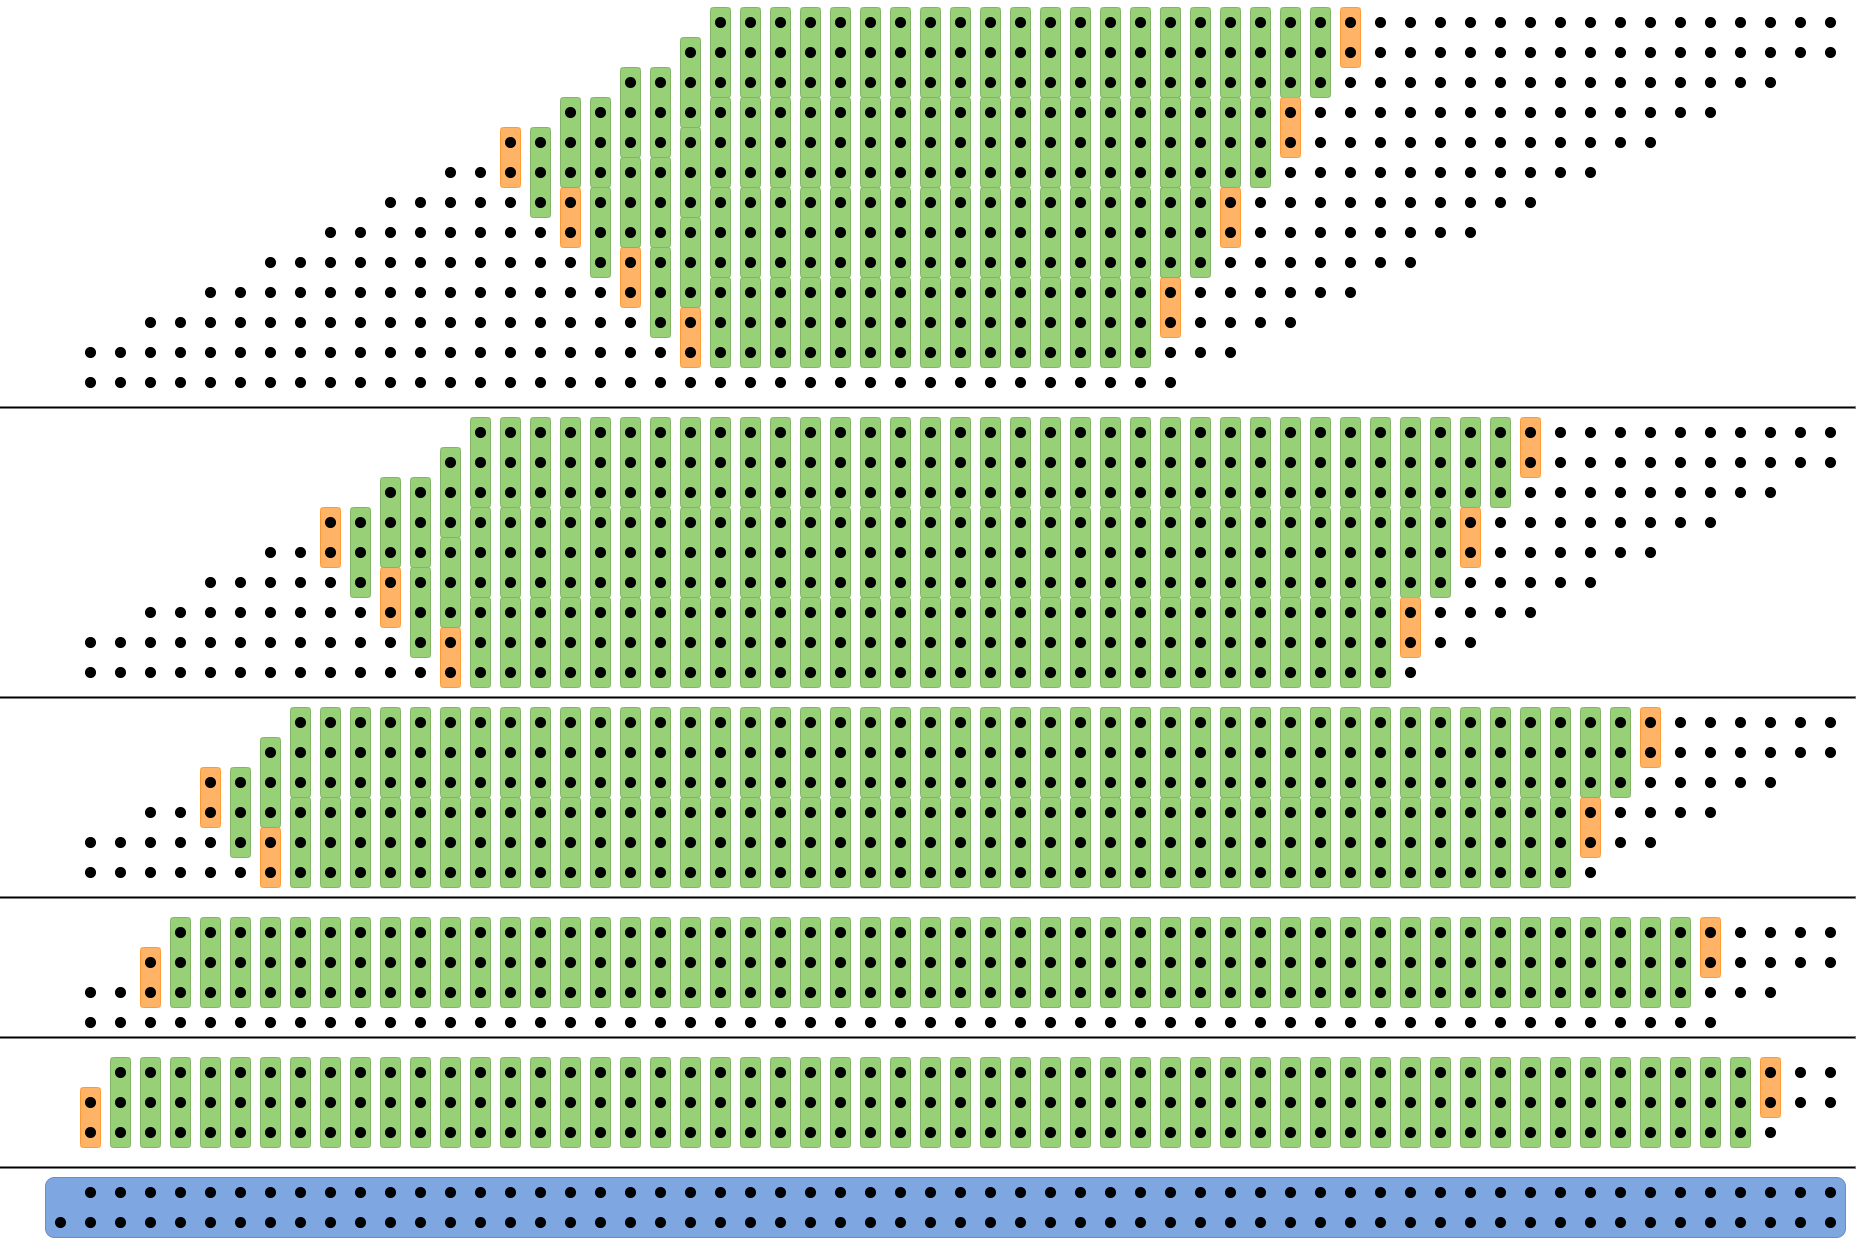
\includegraphics[width=1\textwidth]{Dadda_Tree_2.png}
	\caption{Dadda Tree }
	\label{fig:Dadda_2}
\end{figure}

In \autoref{tab:adders_count} sono riassunti il numero di half-adder e di full-adder per ogni stadio. L'ultimo stadio può essere implementato in diversi modi; per avere un'idea del risultato finale è stato considerato un ripple-carry adder.
\begin{table}[htb]
	\centering
	\begin{tabular}{ccc}
		stage & HA & FA \\ 
		\hline 
		1 & 6 & 33\\ 
		2 & 8 & 84\\ 
		3 & 6 & 105\\ 
		4 & 4 & 90\\ 
		5 & 2 & 51\\ 
		6 & 2 & 55\\ 
		7 & 2 & 58\\ 
		Tot & 30 & 476\\ 
	\end{tabular}  
	\label{tab:adders_count}
	\caption{Number of adders used}
\end{table}
Una volta che è stata definita la struttura ci si è avvalsi di un programma scritto in C++, \footnote{citare}\todo{citare fonte c++} per generare il codice vhdl relativo al MBE multiplier.

\subsubsection{Testbench}
